%%%%%%%%%%%%%%%%%%%%%%%%%%%%%%%%%%%%%%%%%
% Masters/Doctoral Thesis 
% LaTeX Template
% Version 2.4 (22/11/16)
%
% This template has been downloaded from:
% http://www.LaTeXTemplates.com
%
% Version 2.x major modifications by:
% Vel (vel@latextemplates.com)
%
% This template is based on a template by:
% Steve Gunn (http://users.ecs.soton.ac.uk/srg/softwaretools/document/templates/)
% Sunil Patel (http://www.sunilpatel.co.uk/thesis-template/)
%
% Template license:
% CC BY-NC-SA 3.0 (http://creativecommons.org/licenses/by-nc-sa/3.0/)
%
%%%%%%%%%%%%%%%%%%%%%%%%%%%%%%%%%%%%%%%%%

%----------------------------------------------------------------------------------------
%	PACKAGES AND OTHER DOCUMENT CONFIGURATIONS
%----------------------------------------------------------------------------------------

\documentclass[
    11pt, % The default document font size, options: 10pt, 11pt, 12pt
    %oneside, % Two side (alternating margins) for binding by default, uncomment to switch to one side
    english, % ngerman for German
    onehalfspacing, % Single line spacing, alternatives: onehalfspacing or doublespacing
    %draft, % Uncomment to enable draft mode (no pictures, no links, overfull hboxes indicated)
    %nolistspacing, % If the document is onehalfspacing or doublespacing, uncomment this to set spacing in lists to single
    liststotoc, % Uncomment to add the list of figures/tables/etc to the table of contents
    %toctotoc, % Uncomment to add the main table of contents to the table of contents
    parskip, % Uncomment to add space between paragraphs
    nohyperref, % Uncomment to not load the hyperref package
    headsepline, % Uncomment to get a line under the header
    chapterinoneline, % Uncomment to place the chapter title next to the number on one line
    consistentlayout, % Uncomment to change the layout of the declaration, abstract and acknowledgements pages to match the default layout
]{MastersDoctoralThesis} % The class file specifying the document structure

\usepackage[utf8]{inputenc} % Required for inputting international characters
\usepackage[T1]{fontenc} % Output font encoding for international characters

\usepackage{palatino} % Use the Palatino font by default

\usepackage[backend=bibtex,style=ieee,natbib=true,block=space]{biblatex} % Use the bibtex backend with the authoryear citation style (which resembles APA)

\addbibresource{ref.bib} % The filename of the bibliography

\usepackage[autostyle=true]{csquotes} % Required to generate language-dependent quotes in the bibliography

\usepackage{multirow}
\usepackage{makecell}

\usepackage[inline]{enumitem}
\usepackage{array}

\usepackage{rotating}

\usepackage{lipsum}

\usepackage{amsmath}
\usepackage{amssymb}
\usepackage{bbm}

%\usepackage{mhchem}
\usepackage{tensor}

\usepackage{chngcntr}
 
%remove chapter number
%\counterwithout{figure}{chapter}
%\counterwithout{table}{chapter}

%\usepackage[table,xcdraw]{xcolor}
%\usepackage{booktabs}
\usepackage[linesnumbered,ruled,vlined]{algorithm2e}
\usepackage{verbatim} 
\usepackage{mathtools}
%\usepackage{subfig}

%%% ===== My packages =====
\usepackage[utf8]{inputenc}
\usepackage{listings}
\usepackage{amsmath}
\usepackage{physics}
\usepackage{graphicx}
\usepackage{bm}
\usepackage{booktabs}
\usepackage{tabularx}
\usepackage{caption}
\usepackage{subcaption}
\usepackage[colorlinks=true,linkcolor=blue]{hyperref}

%----------------------------------------------------------------------------------------
%	MARGIN SETTINGS
%----------------------------------------------------------------------------------------

\geometry{
	paper=a4paper, % Change to letterpaper for US letter
	inner=2.5cm, % Inner margin
	outer=3.8cm, % Outer margin
	bindingoffset=.5cm, % Binding offset
	top=1.5cm, % Top margin
	bottom=1.5cm, % Bottom margin
	%showframe, % Uncomment to show how the type block is set on the page
}

%----------------------------------------------------------------------------------------
%	THESIS INFORMATION
%----------------------------------------------------------------------------------------

\thesistitle{Embedding Memory into Advanced Dialogue Management} % Your thesis title, this is used in the title and abstract, print it elsewhere with \ttitle

\author{Chia-An \textsc{YU}} % Your name, this is used in the title page and abstract, print it elsewhere with \authorname

\supervisor{Claudiu \textsc{Musat}} % Your supervisor's name, this is used in the title page, print it elsewhere with \supname

\professor{Martin \textsc{Jaggi}} % Your professor's name, this is used in the title page, print it elsewhere with \profname

\examiner{} % Your examiner's name, this is not currently used anywhere in the template, print it elsewhere with \examname

% \degree{Master in Computer Science} % Your degree name, this is used in the title page and abstract, print it elsewhere with \degreename

% \addresses{} % Your address, this is not currently used anywhere in the template, print it elsewhere with \addressname

% \subject{Subject} % Your subject area, this is not currently used anywhere in the template, print it elsewhere with \subjectname

% \keywords{Keyword} % Keywords for your thesis, this is not currently used anywhere in the template, print it elsewhere with \keywordnames

\university{\href{https://www.epfl.ch/index.en.html}{École Polytechnique Fédérale de Lausanne}} % Your university's name and URL, this is used in the title page and abstract, print it elsewhere with \univname

\department{\href{https://www.epfl.ch/schools/ic}{School of Computer and Communication Sciences}} % Your department's name and URL, this is used in the title page and abstract, print it elsewhere with \deptname

\group{\href{https://www.swisscom.ch/}{Swisscom Digital Lab}} % Your research group's name and URL, this is used in the title page, print it elsewhere with \groupname

\faculty{\href{https://www.epfl.ch/labs/mlo/}{Machine Learning and Optimization Laboratory}} % Your faculty's name and URL, this is used in the title page and abstract, print it elsewhere with \facname

%\AtBeginDocument{
%\hypersetup{pdftitle=\ttitle} % Set the PDF's title to your title
%\hypersetup{pdfauthor=\authorname} % Set the PDF's author to your name
%\hypersetup{pdfkeywords=\keywordnames} % Set the PDF's keywords to your keywords
%}

\begin{document}


\frontmatter % Use roman page numbering style (i, ii, iii, iv...) for the pre-content pages

\pagestyle{plain} % Default to the plain heading style until the thesis style is called for the body content

%----------------------------------------------------------------------------------------
%	TITLE PAGE
%----------------------------------------------------------------------------------------

\begin{titlepage}
\begin{center}

\vspace*{-2cm}
\begin{minipage}[c]{0.4\textwidth}
    \begin{flushleft}
        \hspace*{0.4cm}
        
\includegraphics[height=2.0cm]{figures/EPFL_Logo.png}
    \end{flushleft}
\end{minipage}
\hfill
\begin{minipage}[c]{0.4\textwidth}
    \begin{flushright}
        
\includegraphics[height=2.0cm]{figures/Swisscom_Horizontal_RGB_Colour_Navy.png}
        \hspace*{0.4cm}
    \end{flushright}
\end{minipage}
% \vspace*{5.0cm}
\vfill

% \vspace*{.06\textheight}
% {\scshape \Large \univname\par}\vspace{1.5cm} % University name
% \textsc{\Large Master Thesis}\\[0.5cm] % Thesis type

\HRule \\[0.4cm] % Horizontal line
{\huge \bfseries \ttitle\par}\vspace{0.4cm} % Thesis title
\HRule \\[1.5cm] % Horizontal line
 
\textsc{\Large Master Thesis}\\[0.1cm] % Thesis type
{\small Spring Semester 2019}\\
\vfill
 
{\large\emph{Author: }\authorname}\\[0.5cm]
{\small \facname}\\[0.1cm]
{\small\deptname} \\[0.1cm]
{\small \univname} \\[0.1cm]
{\small \groupname}\\[0.1cm]
% \href{https://www.epfl.ch/index.en.html}{EPFL} \\[1cm]
\vfill
 
 
{\large\emph{Professor: } \profname}\\[0.5cm]
% \vspace{0.5cm}
{\large\emph{Supervisor: } \supname}\\

\vfill
% \begin{minipage}[t]{0.45\textwidth}
% \begin{flushleft} \large
% \emph{Author:}\\
% \authorname\\
% % ~\\
% % ~\\
% % \vspace{1cm}
% % \deptname \\
% % \href{https://www.epfl.ch/index.en.html}{EPFL} \\[1cm]
% \end{flushleft}
% \end{minipage}
% \begin{minipage}[t]{0.45\textwidth}
% \begin{flushright} \large
% \emph{Supervisor:} \\
% \supname \\
% \vspace{0.5cm}
% \emph{Assistant:} \\
% \profname \\
% % \vspace{0.5cm}
% % \groupname\\
% \end{flushright}
% \end{minipage}\\[1.5cm]
 
%\vfill

% \large \textit{A thesis submitted in fulfillment of the requirements\\ for the degree of \degreename}\\[0.3cm] % University requirement text
% \textit{in the}\\[0.4cm]

 % Research group name and department name
 
\vfill

%{\large \today}\\[1cm] % Date
{\large August 15, 2019}\\[1cm] % Date

% \vfill

% \includegraphics[width=3cm]{Figures/SDSC_logo.png}\\
% \hspace{0.5cm}
\includegraphics[width=3cm]{EPFL_Logo.png} % Logo

\end{center}
\end{titlepage}


%----------------------------------------------------------------------------------------
%	DECLARATION PAGE
%----------------------------------------------------------------------------------------

% \begin{declaration}
% \addchaptertocentry{\authorshipname} % Add the declaration to the table of contents
% \noindent I, \authorname, declare that this thesis titled, \enquote{\ttitle} and the work presented in it are my own. I confirm that:

% \begin{itemize} 
% \item This work was done wholly or mainly while in candidature for a research degree at this University.
% \item Where any part of this thesis has previously been submitted for a degree or any other qualification at this University or any other institution, this has been clearly stated.
% \item Where I have consulted the published work of others, this is always clearly attributed.
% \item Where I have quoted from the work of others, the source is always given. With the exception of such quotations, this thesis is entirely my own work.
% \item I have acknowledged all main sources of help.
% \item Where the thesis is based on work done by myself jointly with others, I have made clear exactly what was done by others and what I have contributed myself.\\
% \end{itemize}
 
% \noindent Signed:\\
% \rule[0.5em]{25em}{0.5pt} % This prints a line for the signature
 
% \noindent Date:\\
% \rule[0.5em]{25em}{0.5pt} % This prints a line to write the date
% \end{declaration}

\cleardoublepage

%----------------------------------------------------------------------------------------
%	QUOTATION PAGE
%----------------------------------------------------------------------------------------

% \vspace*{0.2\textheight}

% \noindent\enquote{\itshape Thanks to my solid academic training, today I can write hundreds of words on virtually any topic without possessing a shred of information, which is how I got a good job in journalism.}\bigbreak

% \hfill Dave Barry

%----------------------------------------------------------------------------------------
%	ACKNOWLEDGEMENTS
%----------------------------------------------------------------------------------------

%\include{Chapters/Acknowledgements_main}

%----------------------------------------------------------------------------------------
%	ABSTRACT PAGE
%----------------------------------------------------------------------------------------

\begin{abstract}
Frame tracking is a way to embed memory into a dialogue system. Inspired by how human resolves frame references, we propose a new model with an attention mechanism. We also devise a new method to generate synthetic frame tracking data. Empirical analyses show that our method improves accuracy by 6.7 percentage points and shortens training time.
\end{abstract}

%----------------------------------------------------------------------------------------
%	LIST OF CONTENTS/FIGURES/TABLES PAGES
%----------------------------------------------------------------------------------------

\tableofcontents % Prints the main table of contents

\listoffigures % Prints the list of figures

\listoftables % Prints the list of tables

%----------------------------------------------------------------------------------------
%	ABBREVIATIONS
%----------------------------------------------------------------------------------------

%\begin{abbreviations}{ll} % Include a list of abbreviations (a table of two columns)

%\textbf{LAH} & \textbf{L}ist \textbf{A}bbreviations \textbf{H}ere\\ 
%\textbf{WSF} & \textbf{W}hat (it) \textbf{S}tands \textbf{F}or\\

%\end{abbreviations}

%----------------------------------------------------------------------------------------
%	PHYSICAL CONSTANTS/OTHER DEFINITIONS
%----------------------------------------------------------------------------------------

% \begin{constants}{lr@{${}={}$}l} % The list of physical constants is a three column table

% % The \SI{}{} command is provided by the siunitx package, see its documentation for instructions on how to use it

% Speed of Light & $c_{0}$ & \SI{2.99792458e8}{\meter\per\second} (exact)\\
% %Constant Name & $Symbol$ & $Constant Value$ with units\\

% \end{constants}

%----------------------------------------------------------------------------------------
%	SYMBOLS
%----------------------------------------------------------------------------------------

% \begin{symbols}{lll} % Include a list of Symbols (a three column table)

% $a$ & distance & \si{\meter} \\
% $P$ & power & \si{\watt} (\si{\joule\per\second}) \\
% %Symbol & Name & Unit \\

% \addlinespace % Gap to separate the Roman symbols from the Greek

% $\omega$ & angular frequency & \si{\radian} \\

% \end{symbols}

%----------------------------------------------------------------------------------------
%	DEDICATION
%----------------------------------------------------------------------------------------

%\dedicatory{For/Dedicated to/To my\ldots} 

%----------------------------------------------------------------------------------------
%	THESIS CONTENT - CHAPTERS
%----------------------------------------------------------------------------------------

\mainmatter % Begin numeric (1,2,3...) page numbering

\pagestyle{thesis} % Return the page headers back to the "thesis" style

% Include the chapters of the thesis as separate files from the Chapters folder
% Uncomment the lines as you write the chapters

\date{August 15, 2019}
\maketitle

\chapter{Introduction}
Dialogue based assistants, also known as chatbots, are becoming increasingly popular. As improvements in machine learning help us better understand the nuances of natural language, dialogue systems can accomplish more and more complex tasks. 

Existing implementations of dialogue systems are most often goal-oriented and help the user perform a specific task like booking a train ticket or reserving a table.
A goal-oriented dialogue system is like an interface between user and database. When a user knows exactly what he wants, the workflow is straightforward: the system extracts information from user's requests, translate it into database query, and return results to the user. However, this does not work for users who want to explore different options and even compare them, which could happen in many situations such as booking hotels or flights. The reason is that the system keeps only the latest information and loses previous ones when a user changes his mind.

The frame tracking task is proposed to solve this problem \cite{asri2017frames}. In frame tracking, the system maintains a list of frames during a dialogue. A frame is the context for the current turn, or in other words, a summary of a discussion in a dialogue. For example, in a dialogue about booking a traveling package, a frame may contain the price, the number of people, check-in and check-out date, etc., as shown in Table \ref{tab:ex-frame}.
\begin{table}
    \centering
    \caption[An example of a frame]{An example of a frame.}
    \label{tab:ex-frame}
    \begin{tabular}[t]{ll}
        \toprule
        Slot & Value \\
        \midrule
        Budget & 21.3 \\
        Origin city & Kochi \\
        Destination city & Denver \\
        \# adults & 2 \\
        \# children & 6 \\
        Duration & 7 \\
        Start date & August 27 \\
        End date & September 1 \\
        Category & 4.0 \\
        Price & 19028.93 \\
        \bottomrule
    \end{tabular}
\end{table}
%While keeping such list in memory is easy,
The main idea of frame tracking is to make use of this information to improve the system. For each turn in a dialogue, the system finds out the frames related to the current utterance and create frame references.
%At any point of a dialogue, the system chooses one frame to be an active frame, i.e. the frame that is most relevant to the current discussion.
As the conversation goes on, the system may create new frames or change the referred frames. If we consider the list of frames as the memory of the system, the two operations are like storing into and retrieving from memory.

In this paper, we focus on the problem of predicting frame reference. The input of the problem consists of two parts: one is a list of frames $F = \{f_1,\dotsc,f_n\}$ representing the dialogue history, the other is a natural language understanding (NLU) label of the current utterance. The output is the predicted frame reference, which should be a frame $f_i$ in the list $F$ indicating that this is the frame most related to the label.

Previous research \cite{schulz2017frame} on frame tracking uses recurrent neural networks (RNN) to encode frames into vectors. However, this ignores the fact that each slot-value pair has different importance when the reference NLU label is different. For example, when the label is a location, the destination city and origin city slots should be more important than the number of people when we try to find the most relevant frame. Therefore, we propose a new model that uses an attention mechanism to account for this.

Another challenge of frame tracking is the limited amount of available data. The only dataset that has frame tracking labels is FRAMES \cite{asri2017frames}, which only has 1369 dialogues. This is relatively small comparing to other benchmark dialogue datasets. So we come up with a method to create synthetic frame tracking data using large dialogue datasets that don't have frame tracking labels.


\section{Related work}
Recently, researches start to develop memory-enhanced dialogue systems.
In addition to creating extra frame tracking component to the dialogue system, some methods focus on incorporating memory into existing components such as slot filling and state tracking. Chen et al. \cite{chen2016end} used RNN to encode contextual sentences, which are further encoded using an attention mechanism to enhance the language understanding tagging sequence. Several pieces of research work on improving state tracking: Lee et al. \cite{lee2016task} work at the semantic level, i.e. representing each turn as the NLU results, while Sharma et al. \cite{sharma2019improving} use the textual content directly. Perez et al. \cite{perez2016dialog} approach this problem differently. They formulate state tracking as a question-answering problem and use MemN2N \cite{weston2014memory} to model the memory.

%state tracking review 15
%-MACHINE LEARNING FOR DIALOG STATE TRACKING - A REVIEW

%*transfer learning
%Goal-Oriented Chatbot Dialog Management Bootstrapping with Transfer Learning

%GLOBAL-TO-LOCAL MEMORY POINTER NETWORKS FOR TASK-ORIENTED DIALOGUE???



\chapter{Frame tracking}
\section{FRAMES dataset}

FRAMES dataset is created specifically for the frame tracking task. Its dialogues are longer and more complicated comparing to the ones in other datasets, and there are special labels for frame tracking. The dialogues were collected in a wizard-of-oz fashion: two people playing the role of user and system, with the user having a goal hidden from the system, and with the system having a database unknown to the user \cite{kelley1984iterative, rieser2005corpus, wen2016network}. The users' tasks are designed so that users have to go back-and-forth between options to achieve their goal and thus creates complicated dialogue structures.
% what is action, slot, value?
For each utterance, there are annotations of NLU labels, i.e. action, slot, and value, and an optional frame reference label if this action-slot-value tuple is related to a previous frame. The frame is then represented as a list of slot-value pairs.

% user turn only? A: mention in experiment
The frame references appearing in FRAMES can be categorized into three types: explicit, anaphora, and implicit. Explicit reference is when the NLU label appears in the referred frame, i.e. the user mentions a slot value explicitly. Reference using anaphora is similar except that the user uses anaphora instead of a slot value. The problem of resolving this kind of reference is closely related to the coreference resolution in dialogues. Implicit reference happens when the utterance itself contains no clue and the reference depends heavily on the context of the dialogue. In such cases, the referred frame is usually the one mentioned in the previous turn.

Here are some examples of each type of frame reference. The slot values having a reference are in bold.
\begin{itemize}
    \item Explicit: a detailed example is in Table \ref{tab:ex-explicit}.
    \begin{itemize}
        \item How many days would I be in \textbf{Kobe}? %(dial id = 1, turn id = 12)
        \item Ok, I would like to purchase the trip with the \textbf{4 star} hotel. %(dial id = 4, turn id = 6)
    \end{itemize}

    \item Anaphora: a detailed example in Table \ref{tab:ex-anaphora}.
    \begin{itemize}
        \item No, \textbf{that}'s too far for me. I need a flight that leaves from Birmingham. %(dial id = 1, turn id = 10)
        \item Ok, then I would like to purchase \textbf{this package}. What activities are included in this package? %(dial id = 1, turn id = 16)
    \end{itemize}
    
    \item Implicit: without context, these might look the same as explicit references. The difference is that the slots and values here do not appear in any existing frames thus can not be explicit references. A detailed example is in Table \ref{tab:ex-implicit}.
    \begin{itemize}
        \item{
            %SYSTEM: Yes, I do. I have one for 8445.37 USD. Would you like to book this package? The guest rating is 7.15 / 10 and ... at 1:00 a.m.
            Is \textbf{breakfast} included? %(dial id = 3, turn id = 8)
        }
        \item{
            %SYSTEM: Ok. I can upgrade your flights to business class for a total of 2715.60 USD. Would you like that?
            Yes perfect. How is the \textbf{hotel}? %(dial id = 33, turn id = 6)
        }
        \item{
            %SYSTEM: Okay, our best deal in Santos is a 7 day trip at a 3.5 star hotel near a museum and a palace.
            Reasonable. Any free \textbf{wifi} for the kids? %(dial id = 1191, turn id = 4)
        }
    \end{itemize}
\end{itemize}

%[explain detailed example]
%[frame reference can be far]

\begin{table}
    \centering
    \caption[Explicit frame reference]{An example of explicit frame reference. The frames are in Table \ref{tab:ex-explicit-frames}.}
    \label{tab:ex-explicit}
    \begin{tabularx}{\textwidth}{llX|l}
        \toprule
        Turn & Author & Utterance & Remark \\
        \midrule
        1 & User & Hello, I am looking to book a trip for 2 adults and 6 children for \$21,300 or less. We are departing from Kochi for Denver. & Create frame 1 \\
        2 & System & I have several options available within your budget. How long would you like to travel for? And do you have dates in mind? & Update frame 1 \\
        3 & User & I do not have any dates in mind. I would like to spend as much time in Denver as my budget will allow. & Update frame 1 \\
        4 & System & I can book 7 days at a 4.0 star hotel for 19028.93USD. I can also book 7 days at a 3.0 star hotel for 12824.84USD. & Create frame 2 and 3 \\
        5 & User & Do these packages have different departure dates? When would I be leaving for each of them? & \\
        6 & System & The 3.0 star trip leaves Kochi August 26 and returns August 31. The 4.0 star leaves August 27 from Kochi and returns September 1. & Update frame 2 and 3 \\
        7 & User & Ok, I would like to purchase the trip with the \textbf{4-star} hotel. & Refer to frame 2 \\
        \bottomrule
    \end{tabularx}
\end{table}

\begin{table}
    \centering
    \caption[Frames of explicit frame reference]{Frames created in the example dialogue of explicit frame reference (Table \ref{tab:ex-anaphora}).}
    \label{tab:ex-explicit-frames}
    \begin{subtable}[t]{0.48\textwidth}
        \centering
        \caption{Frame 1}
        \begin{tabular}[t]{ll}
            \toprule
            Slot & Value \\
            \midrule
            Intent & book \\
            Budget & 21.3 \\
            Origin city & Kochi \\
            Destination city & Denver \\
            \# adults & 2 \\
            \# children & 6 \\
            Count & several options \\
            Start date & -1 \\
            End date & -1 \\
            Max duration & \$MAX \\
            \bottomrule
        \end{tabular}
    \end{subtable}
    \begin{subtable}[t]{0.48\textwidth}
        \centering
        \caption{Frame 2}
        \begin{tabular}[t]{ll}
            \toprule
            Slot & Value \\
            \midrule
            Intent & book \\
            Budget & 21.3 \\
            Origin city & Kochi \\
            Destination city & Denver \\
            \# adults & 2 \\
            \# children & 6 \\
            Max duration & \$MAX \\
            Duration & 7 \\
            Start date & August 27 \\
            End date & September 1 \\
            Category & 4.0 \\
            Price & 19028.93 \\
            \bottomrule
        \end{tabular}
    \end{subtable}
    
    \vspace{\baselineskip}
    \begin{subtable}[t]{\textwidth}
        \centering
        \caption{Frame 3}
        \begin{tabular}[t]{ll}
            \toprule
            Slot & Value \\
            \midrule
            Intent & book \\
            Budget & 21.3 \\
            Origin city & Kochi \\
            Destination city & Denver \\
            \# adults & 2 \\
            \# children & 6 \\
            Max duration & \$MAX \\
            Duration & 7 \\
            Start date & August 26 \\
            End date & August 31 \\
            Category & 3.0 \\
            Price & 12824.84 \\
            \bottomrule
        \end{tabular}
    \end{subtable}
\end{table}

\iffalse
\begin{table}
    \centering
    %\resizebox{0.5\columnwidth}{!}{
    \begin{subtable}[t]{0.3\textwidth}
        \centering
        %\resizebox{\columnwidth}{!}{
        \begin{tabular}[t]{ll}
            \toprule
            Slot & Value \\
            \midrule
            Intent & book \\
            Budget & 21.3 \\
            Origin city & Kochi \\
            Destination city & Denver \\
            \# adults & 2 \\
            \# children & 6 \\
            Count & several options \\
            Start date & -1 \\
            End date & -1 \\
            Max duration & \$MAX \\
            \bottomrule
        \end{tabular}
        %}
        \caption{Frame 1}
    \end{subtable}
    \hspace{\fill}
    \begin{subtable}[t]{0.3\textwidth}
        \centering
        %\resizebox{\columnwidth}{!}{
        \begin{tabular}[t]{ll}
            \toprule
            Slot & Value \\
            \midrule
            Intent & book \\
            Budget & 21.3 \\
            Origin city & Kochi \\
            Destination city & Denver \\
            \# adults & 2 \\
            \# children & 6 \\
            Max duration & \$MAX \\
            Duration & 7 \\
            Start date & August 27 \\
            End date & September 1 \\
            Category & 4.0 \\
            Price & 19028.93 \\
            \bottomrule
        \end{tabular}
        %}
        \caption{Frame 2}
    \end{subtable}
    \hspace{\fill}
    \begin{subtable}[t]{0.3\textwidth}
        \centering
        %\resizebox{\columnwidth}{!}{
        \begin{tabular}[t]{ll}
            \toprule
            Slot & Value \\
            \midrule
            Intent & book \\
            Budget & 21.3 \\
            Origin city & Kochi \\
            Destination city & Denver \\
            \# adults & 2 \\
            \# children & 6 \\
            Max duration & \$MAX \\
            Duration & 7 \\
            Start date & August 26 \\
            End date & August 31 \\
            Category & 3.0 \\
            Price & 12824.84 \\
            \bottomrule
        \end{tabular}
        %}
        \caption{Frame 3}
    \end{subtable}
    %}
    \caption{Caption}
    \label{tab:ex-frames2}
\end{table}
\fi


\begin{table}
    \centering
    \caption[Anaphora frame reference]{An example of anaphora frame reference. The frames are in Table \ref{tab:ex-anaphora-frames}. The reference in turn 11 and ``the hotel" part in turn 13 is an anaphora, and the ``Fortaleza" in turn 13 is explicit because it directly mentions a slot value.}
    \label{tab:ex-anaphora}
    \begin{tabularx}{\textwidth}{llX|l}
        \toprule
        Turn & Author & Utterance & Remark \\
        \midrule
        1 & User & Hey im looking to check out fortaleza. I'm leaving from Sapporo on August 27 & Create frame 1 \\
        2 & System & Hi there! I can offer you a six-day vacation package starting August 27th for only 3933.10USD. Does this fit within your budget? & Create frame 2 \\
        3 & User & When is the return date? & \\
        4 & System & You would be returning on the 31st of August. & Update frame 2 \\
        5 & User & I would like to travel until September 7, or closer to that date. ... & \\
        %& & & \\
        \vdots & \vdots & \vdots & \vdots \\
        %5 & User & I would like to travel until September 7, or closer to that date. Is there anything available in Frankfurt for that window? & \\
        %6 & System & Unfortunately those are the closest days I can offer you to your specifications. & \\
        %7 & User & What about in Ulsan? & \\
        %8 & System & It looks like every package available is for the 27th - 30th of August, with the best deal being 472.37USD for the trip. & \\
        9 & User & Ok. One last destination I am wondering about. Curitiba - what've you got there? & Create frame 6 \\
        10 & System & How about August 30th - September 6th at the Hotel Leisure? 4234.65USD if you book now. & Create frame 7 \\
        11 & User & I like the sounds of that. What is \textbf{the hotel} like? Any details? & Refer to frame 7 \\
        12 & System & The Hotel Leisure is a 3-star resort with a 6.91/10 guest rating, free breakfast, free wifi and free parking. Would you like me to book this destination? & Update frame 7 \\
        13 & User & What is \textbf{the hotel in Fortaleza} like? & Refer to frame 2 \\
        \bottomrule
    \end{tabularx}
\end{table}

\begin{table}
    \centering
    \caption[Frames of anaphora frame reference]{Frames created in the example dialogue of anaphora frame reference (Table \ref{tab:ex-anaphora}).}
    \label{tab:ex-anaphora-frames}
    \begin{subtable}[t]{0.48\textwidth}
        \centering
        \caption{Frame 1}
        \begin{tabular}[t]{ll}
            \toprule
            Slot & Value \\
            \midrule
            Intent & book \\
            Origin city & Sapporo \\
            Destination city & Fortaleza \\
            Start date & August 27 \\
            \bottomrule
        \end{tabular}
    \end{subtable}
    \begin{subtable}[t]{0.48\textwidth}
        \centering
        \caption{Frame 2}
        \begin{tabular}[t]{ll}
            \toprule
            Slot & Value \\
            \midrule
            Intent & book \\
            Origin city & Sapporo \\
            Destination city & Fortaleza \\
            Start date & August 27 \\
            End date & August 31 \\
            Duration & 6 \\
            Price & 3933.1 \\
            \bottomrule
        \end{tabular}
    \end{subtable}
    
    \vspace{\baselineskip}
    \begin{subtable}[t]{0.48\textwidth}
        \centering
        \caption{Frame 6}
        \begin{tabular}[t]{ll}
            \toprule
            Slot & Value \\
            \midrule
            Intent & book \\
            Origin city & Sapporo \\
            Destination city & Curitiba \\
            Start date & August 27 \\
            \bottomrule
        \end{tabular}
    \end{subtable}
    \begin{subtable}[t]{0.48\textwidth}
        \centering
        \caption{Frame 7}
        \begin{tabular}[t]{ll}
            \toprule
            Slot & Value \\
            \midrule
            Intent & book \\
            Origin city & Sapporo \\
            Destination city & Curitiba \\
            Start date & August 30 \\
            End date & September 6 \\
            Name & Hotel Leisure \\
            Category & 3.0 \\
            Price & 4234.65 \\
            Guest rating & 6.91 \\
            Breakfast & true \\
            Parking & true \\
            Wifi & true \\
            \bottomrule
        \end{tabular}
    \end{subtable}
\end{table}




\begin{table}
    \centering
    \caption[Implicit frame reference]{An example of implicit frame reference. The frames are in Table \ref{tab:ex-implicit-frames}.}
    \label{tab:ex-implicit}
    \begin{tabularx}{\textwidth}{llX|l}
        \toprule
        Turn & Author & Utterance & Remark \\
        \midrule
        1 & User & Hello I am looking to bring my 6 kids and I to Portland and leave from Minneapolis. We can travel whenever and have no budgetary constraints. & Create frame 1 \\
        2 & System & Unfortunately we don't have any available trips to Portland as of right now. Is there another city you can go to? & Update frame 1 \\
        3 & User & Ahh... Let's check Santos then. & Create frame 2 \\
        4 & System & Okay, our best deal in Santos is a 7 day trip at a 3.5 star hotel near a museum and a palace. & Create frame 3 \\
        5 & User & Reasonable. Any \textbf{free wifi} for the kids? & Refer to frame 3 \\
        \bottomrule
    \end{tabularx}
\end{table}

\begin{table}
    \centering
    \caption[Frames of implicit frame reference]{Frames created in the example dialogue of implicit frame reference (Table \ref{tab:ex-implicit}).}
    \label{tab:ex-implicit-frames}
    \begin{subtable}[t]{0.48\textwidth}
        \centering
        \caption{Frame 1}
        \begin{tabular}[t]{ll}
            \toprule
            Slot & Value \\
            \midrule
            Intent & book \\
            Origin city & Minneapolis \\
            Destination city & Portland \\
            \# children & 6 \\
            Start date & -1 \\
            Budget & -1 \\
            No result & true \\
            \bottomrule
        \end{tabular}
    \end{subtable}
    \begin{subtable}[t]{0.48\textwidth}
        \centering
        \caption{Frame 2}
        \begin{tabular}[t]{ll}
            \toprule
            Slot & Value \\
            \midrule
            Intent & book \\
            Origin city & Minneapolis \\
            Destination city & Santos \\
            \# children & 6 \\
            Start date & -1 \\
            Budget & -1 \\
            \bottomrule
        \end{tabular}
    \end{subtable}
    
    \vspace{\baselineskip}
    \begin{subtable}[t]{\textwidth}
        \centering
        \caption{Frame 3}
        \begin{tabular}[t]{ll}
            \toprule
            Slot & Value \\
            \midrule
            Intent & book \\
            Origin city & Minneapolis \\
            Destination city & Santos \\
            \# children & 6 \\
            Start date & -1 \\
            Budget & -1 \\
            Category & 3.5 \\
            Duration & 7 \\
            Museum & true \\
            Palace & true \\
            \bottomrule
        \end{tabular}
    \end{subtable}
\end{table}


\section{Synthetic dataset}
\label{sec:syn}
The amount of data in FRAMES is limited. To have more training data for frame tracking, we generate synthetic dialogues that have a similar structure as the ones in FRAMES. More precisely, we create actions of switching frame reference by interleaving multiple simple dialogues.

% what is interleaving (still hard to understand...)
The operation of interleaving a set of dialogues is defined as follows. For each user turn, the utterance is chosen from any dialogue in the set, and utterance of the following system turn is the response to the corresponding user utterance. The chosen dialogue can be arbitrary in each user turn, but the turns should be taken in the same order as in the original dialogue. The result is as if multiple users were talking to the system at the same time.
This is an effective way to create artificial frame switching actions because there is a context switch whenever we choose a dialogue that is different from the source of the previous turn. However, such switches can be ambiguous if dialogues are chosen arbitrarily in each turn. Some turns do not have enough information themselves to identify a frame without context. If those turns are placed after another turn from a different dialogue, it might be impossible to find out the referred frame or even notice a switch exists.
% how to interleave (mixable turn) (identifying turn)
To avoid this problem, we define the notion of identifying turn. An identifying turn is a turn that has explicit mention of slot values in its referred frame. When interleaving dialogues, we switch dialogues only at identifying turns.

% how to create frames labels
% how to create frame references
The frame label of the interleaved dialogue can be easily obtained from the source dialogues: if a new frame is created in a turn of source dialogue, the same frame is created in the corresponding turn in the interleaved dialogue. Similarly, for each slot-value in the utterance of interleaved dialogue, the frame reference is copied directly from its source dialogue.

%\subsection{MultiWOZ dataset}
%MultiWOZ: large, multiple domain, multidomain dialogue, state of each turn
The dataset we use to create synthetic data is MultiWOZ 2.0 \cite{budzianowski2018multiwoz}.
%MultiWOZ is the dataset we use to create synthetic data.
It is a large scale goal-oriented dataset created for multi-domain dialogue modeling. It consists of about 10,000 dialogues and covers a wide range of domains, including restaurant, train, hotel, etc. It has both single domain dialogue and multi-domain dialogue. Despite having rich content, it only has dialogue state label for every two turns (user turn and system turn) and no annotation of frames so we have to convert the labels into frame labels.
%We use heuristic rules described in Algorithm (...) to transform states into frames.
We then take the single domain dialogues along with their frame labels and interleave them to generate synthetic datasets.
We generate one synthetic dialogue by interleaving two dialogues. The two dialogues are in the same domain for the first synthetic dataset, and the domains are different for the other two synthetic datasets. More information on the three synthetic datasets we generated are listed in Table \ref{tab:syn}.

%[Algorithm that transforms states to frames]

\begin{table}
    \centering
    \caption[Synthetic datasets]{Synthetic datasets.}
    \label{tab:syn}
    \begin{tabular}{lrl}
        \toprule
         & \# dialogues & Domain(s) \\
        \midrule
        FRAMES & 1369 & Hotel + flight \\
        Synthetic 1 & 5488 & Single domain \\
        Synthetic 2 & 3820 & Hotel + restaurant \\
        Synthetic 3 & 3820 & Hotel + transportation (taxi and train) \\
        \bottomrule
    \end{tabular}
\end{table}



\chapter{Methodology}
\section{Model}
%[dimension]
Our proposed model consists mainly of two parts: one is an NLU label encoder, and the other is a frame encoder. The two encoders produce a vector for the corresponding part of the input. We use a dot product to compute the similarity score between an NLU label and a frame. The output is a probability distribution over all candidate frames computed by taking softmax of all the similarity scores of the frames. Softmax is a kind of normalization that transforms a real vector into a discrete probability distribution. It is defined as
\begin{equation}\label{eq:softmax}
    \text{softmax}(x)_i = \frac{\exp(x_i)}{\sum_{j = 1}^{n}{\exp(x_j)}} \text{, for } i = 1 \dotsc n\,.
\end{equation}
The high-level overview of the model architecture is in Figure \ref{fig:main}.

\begin{figure}
    \centering
    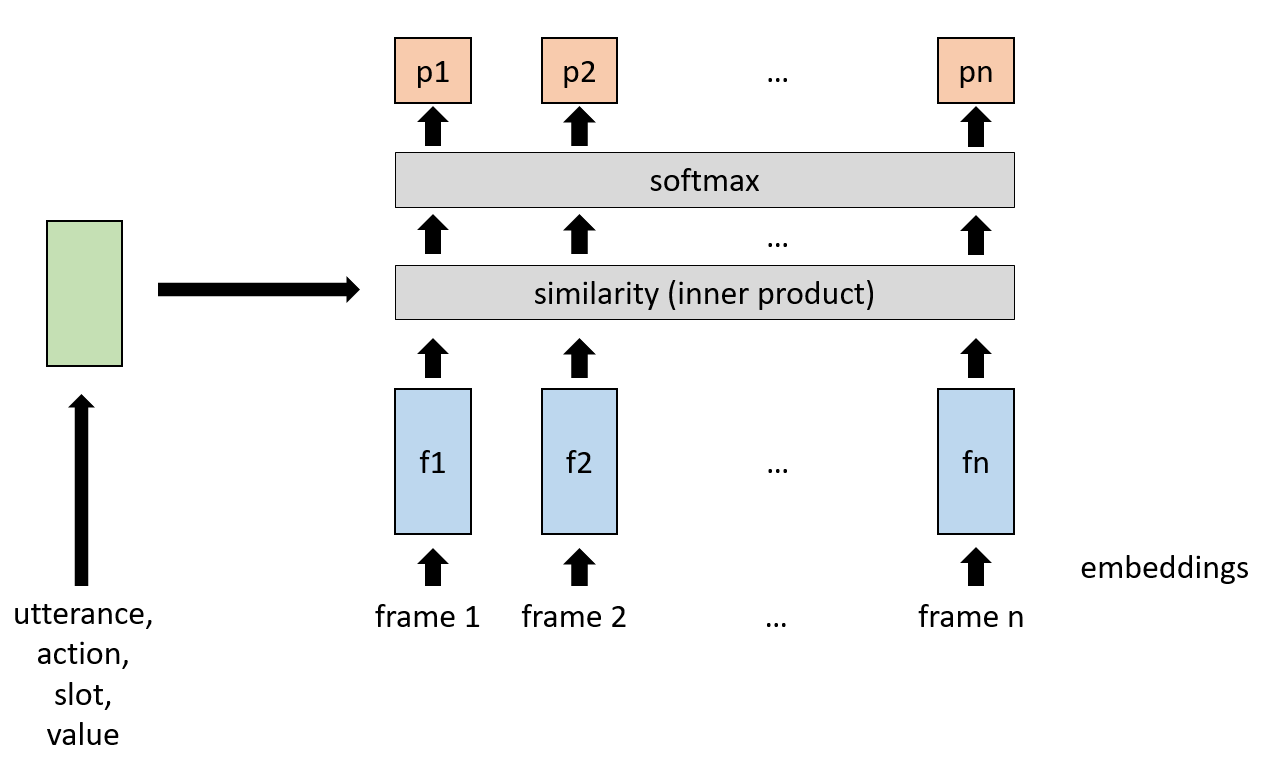
\includegraphics[width=\columnwidth]{figures/main.png}
    \caption[Model architecture]{Model architecture. The green block on the left is NLU label encoder (Figure \ref{fig:nlu-label}). The blue blocks at the bottom are frame encoders (Figure \ref{fig:frame}).}
    \label{fig:main}
\end{figure}

\subsection{Embedding of input}
Both NLU label encoder and frame encoder use text embedding and token embedding to convert structured input into vectors. The embeddings are shared between the two encoders. There are three embeddings: text embedding, act embedding, slot embedding. The act embedding and slot embedding are very similar. We treat each act and slot as a unique token and assign them a trainable embedding vector. The text embedding is used to embed slot values. 

% letter trigram, BERT feature
We use two different text embedding models. The first one, shown in Figure \ref{fig:bert}, is based on a pre-trained BERT \cite{devlin2018bert} feature. We use a uncased 12-layered BERT model\footnote{\url{https://github.com/huggingface/pytorch-transformers}}. The embedding of a slot value is the average of the last layer. We use a linear projection to adjust the dimension of the embedding so that it is compatible with the other part of the model.

\begin{figure}
    \centering
    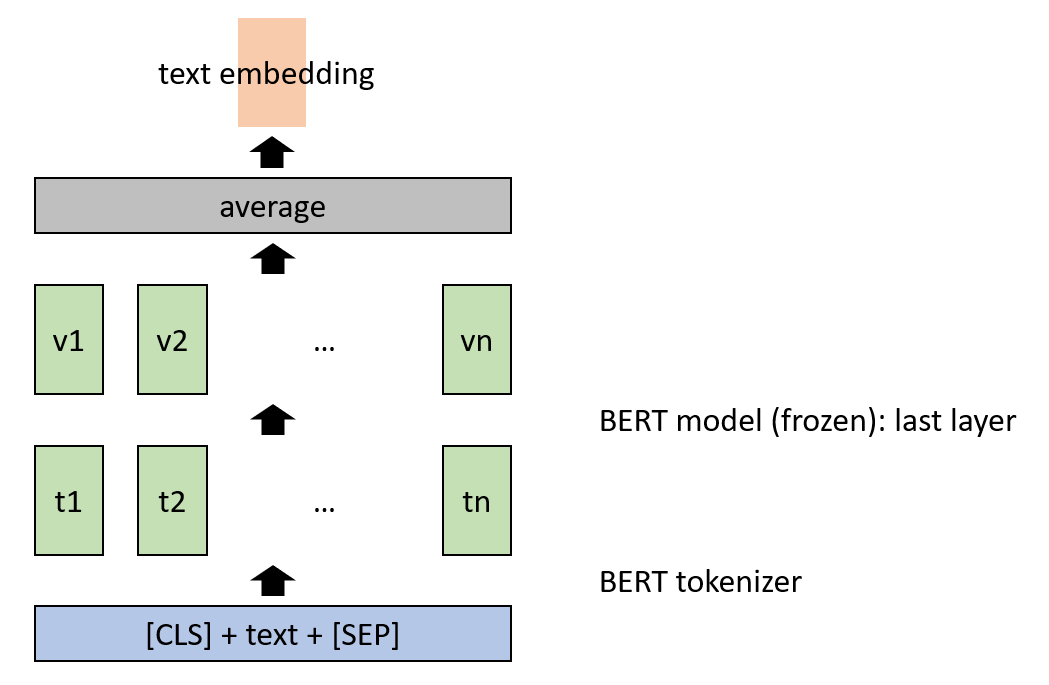
\includegraphics[width=\columnwidth]{figures/bert.png}
    \caption[Text embedding using pre-trained BERT]{Architecture of text embedding using pre-trained BERT.}
    \label{fig:bert}
\end{figure}

The other text embedding is based on letter trigram and RNN (Figure \ref{fig:gru}. We first tokenize the text using nltk's TweetTokenizer\footnote{\url{https://www.nltk.org/}} and split each token into letter trigrams. For example, the list of letter trigram of ``hotel" is ``\#ho", ``hot", ``ote", ``tel", and ``el\#". We assign each trigram to a trainable embedding vector. The embedding of a token is then the sum of embedding of its trigrams. We then use a bidirectional GRU to encode all tokens into one vector. The final embedding is the concatenation of forward and backward hidden state of the GRU.

\begin{figure}
    \centering
    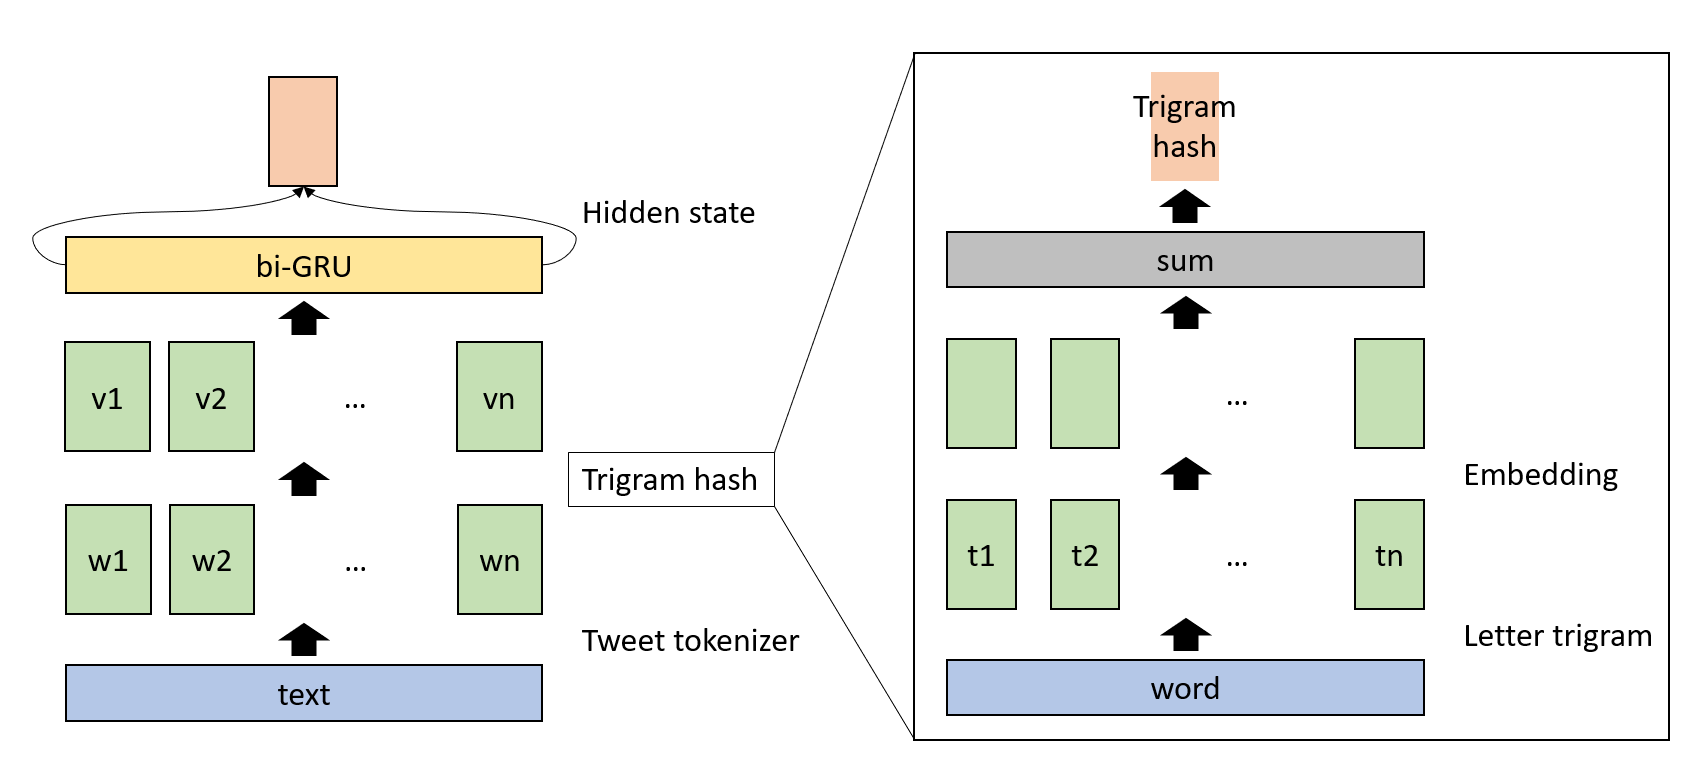
\includegraphics[width=\columnwidth]{figures/lstm.png}
    \caption[Text embedding using letter trigram and GRU]{Architecture of text embedding using letter trigram and GRU.}
    \label{fig:gru}
\end{figure}


\subsection{NLU label encoder}
This encoder takes as input an act embedding, a slot embedding, and a value embedding. We treat them as a sequence of length three and pass it through a bidirectional GRU. We then concatenate the forward and backward hidden state and project it to have a proper dimension. The architecture is in Figure \ref{fig:nlu-label}.

\begin{figure}
    \centering
    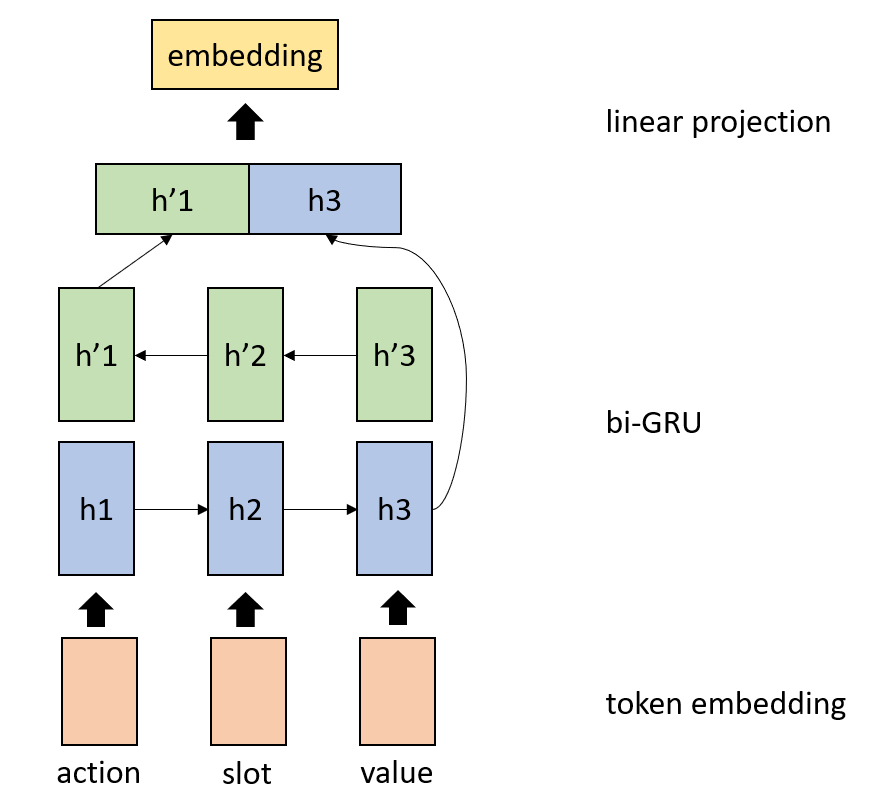
\includegraphics[width=0.7\columnwidth]{figures/utterance.png}
    \caption[NLU label encoder]{Architecture of NLU label encoder.}
    \label{fig:nlu-label}
\end{figure}

\subsection{Frame encoder}
A frame is a list of slot-value pairs. To encode this, we concatenate the slot and value embedding vectors for each slot-value pair and pass the list of concatenated vectors through a bidirectional GRU.

If there is no attention mechanism, we concatenate the forward and backward hidden state of the GRU and use a linear projection to compute the output vector. If an attention mechanism is used, we concatenate the outputs of both direction and project each vector to adjust the dimension. The final output is then the linear combination of the resulting vectors, with coefficients being attention scores normalized by softmax. The architecture with attention mechanism is shown in Figure \ref{fig:frame}.

\begin{figure}
    \centering
    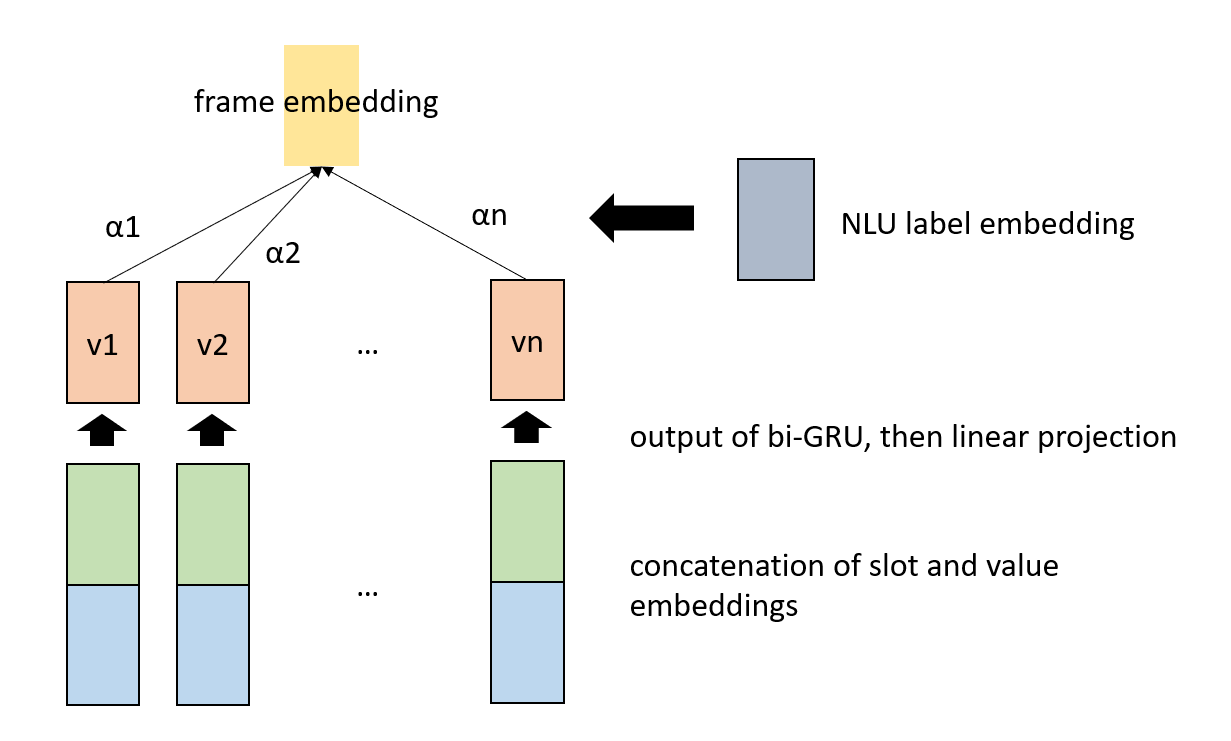
\includegraphics[width=\columnwidth]{figures/frames.png}
    \caption[Frame encoder]{Architecture of frame encoder.}
    \label{fig:frame}
\end{figure}

The detailed formula of each attention mechanism is in Table \ref{tab:att}. In addition to an encoded frame, most of the attention mechanisms we use also take an encoded NLU label as input so that the attention score is adapted for different situations. The only exception is the content-based attention, which computes the score using only the content of slot-values of the given frame.

%[more on attention]
% with query or not

\begin{table}
    \caption[Formulas of attention mechanisms]{Formulas of attention mechanisms. $x$ is the embedding of a NLU label, $y$ is an the embedding of a slot-value pair in a frame, $d_y$ is the dimension of $y$, and $d_k$ is the dimension of $W_ky$. $w$, $W$, $W_k$, $W_q$, and $b$ are trainable parameters.}
    \label{tab:att}
    \centering
    \begin{tabular}{ll}
        \toprule
        Type & Formula for $\alpha$ (attention score) \\
        \midrule
        Content-based & $\tanh(wy+b)$ \\
        Dot-product & $x^Ty$ \\
        Cosine & $x^Ty\ /\ \norm{x}\norm{y}$ \\
        General & $x^TWy$ \\
        Query-key & $(W_qx)^TW_ky$ \\
        Scaled dot-product & $x^Ty / \sqrt{d_y}$ \\
        %Scaled general & $x^TWy / \sqrt{d_y}$ \\
        Scaled query-key & $(W_qx)^TW_ky / \sqrt{d_k}$ \\
        \bottomrule
    \end{tabular}
\end{table}



\chapter{Experiments}
\section{Settings} \label{section:setting}
We train the proposed model using the setting described below. FRAMES dataset comes with a predefined 10-fold split. We use the first eight folds for training, the ninth fold for validation, and the tenth fold for testing. We choose Adam \cite{kingma2014adam} as the optimization algorithm with $10^{-4}$ learning rate and $10^{-4}$ weight decay.

We set the batch size to one for the training because the input has nested variable-length lists, which are hard to gather into one batch. We train the model for 10 epochs because it is long enough to have training processes converge. We take the model with the highest validation score and evaluate it on the testing set.

The performance of the model is measured by accuracy. We consider only user turns for evaluation even though system turns are also used for training. The main reason is that there is no need to predict frame reference for system turn in a real-world situation. The same metric is used in \cite{schulz2017frame}. For each experiment, we repeat it with five different random seeds and report the average and the variance of the results.

\section{Comparison with baselines}
\begin{table}
    \centering
    \caption[Accuracy scores of baselines and the proposed model]{Accuracy scores of baselines and the proposed model. We use dot product for the attention mechanism. The result from \cite{schulz2017frame} uses 10-fold cross-validation. ``Shuffle" means that we shuffle the training samples for each epoch, otherwise we use the same order as they appear in a dialogue.}
    \label{tab:baselines}
    \begin{tabular}[t]{lrr}
        \toprule
        Methods & No attention & Attention \\
        \midrule
        % [0.584070796460177, 0.577433628318584, 0.5873893805309734, 0.5741150442477876, 0.5807522123893806]
        Random & $58.1 \pm 0.22$ & - \\
        Maluuba \cite{schulz2017frame} & $76.4 \pm 4.49$ & -\\
        %Maluuba & $76.4 \pm 4.49$ & -\\
        BERT w/o shuffle & $77.5 \pm 0.52$ & $81.0 \pm 0.69$ \\
        GRU w/o shuffle & $79.3 \pm 0.28$ & $81.9 \pm 1.05$ \\
        %\midrule
        BERT w/ shuffle & $81.0 \pm 0.73$ & $82.3 \pm 1.70$ \\
        GRU w/ shuffle & $79.5 \pm 0.65$ & $\bm{82.8 \pm 0.52}$ \\
        \bottomrule
    \end{tabular}
\end{table}

We compare our results with two baselines. The first one is a random baseline. It predicts a frame reference by choosing one from the list of frames uniformly at random. The other baseline is from the authors who proposed this frame tracking task \cite{schulz2017frame}. Their model predicts different types of frame reference at the same time, including slot-based prediction, which is the definition used in this paper.
The results are in Table \ref{tab:baselines}.
%Their model also has encoders for NLU labels and frames, but the architecture of encoders and ...
%similar model, no attention, predict multiple slot-based / act-based at the same time
%random baseline, maluuba baseline with cross validation

The accuracy of the random baseline might seem unreasonably high, given that there could be several frames to choose from. However, this is not true at the beginning of a dialogue, where there are very few, or even one, frame created. As shown in Figure \ref{fig:frames-dist}, about $43\%$ of the samples has only one frame, meaning that predictions of those samples are always correct. This explains why a random model can have an accuracy of over $50\%$. We keep those samples for evaluation so that we can compare our results with other baselines.

\begin{figure}
    \centering
    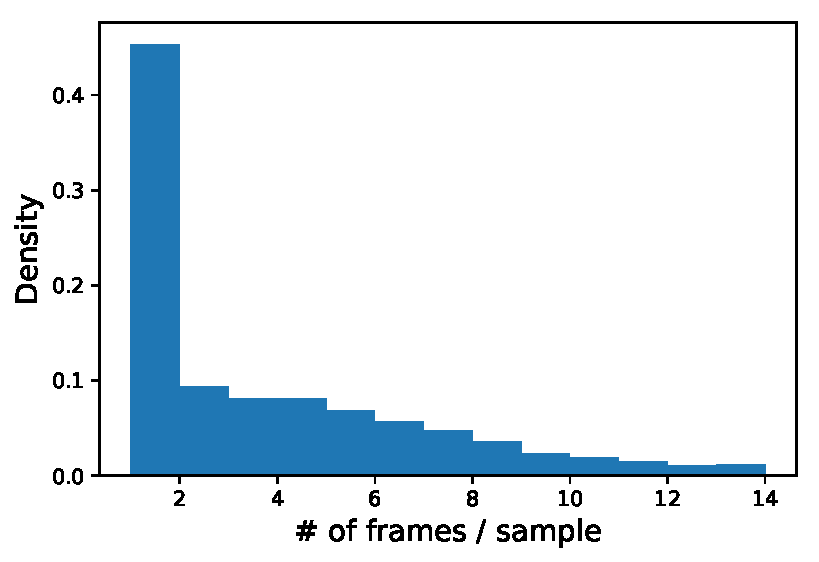
\includegraphics{figures/n_frames_dist.pdf}
    \caption[Distribution of number of frames]{Distribution of number of frames.}
    \label{fig:frames-dist}
\end{figure}

For the proposed model, we can see that it consistently outperforms the two baselines regardless of the configuration.
Also, adding the attention mechanism always improves the accuracy by at least one percentage point. This demonstrates the efficacy of attention mechanisms in the frame tracking task.
Another important point is the effect of shuffling training samples. At first, we train the model without shuffling, i.e. using the same order as they appear in dialogues. However, even with the intrinsic order relation between samples, the training still benefits a lot from shuffling, leading to the best result in Table \ref{tab:baselines}.

%[training time]


\section{Attention mechanisms} \label{sec:att}
\begin{table}
    \centering
    \caption[Accuracy scores of different attention mechanisms]{Accuracy scores of different attention mechanisms.}
    \label{tab:att-res}
    \begin{tabular}[t]{lrr}
        \toprule
        Attention mechanisms & GRU & BERT \\
        \midrule
        No attention & $79.5 \pm 0.65$ & $81.0 \pm 0.73$ \\
        Content-based & $79.6 \pm 1.09$ & $81.9 \pm 0.77$ \\
        Cosine & $80.7 \pm 0.33$ & $81.3 \pm 0.93$ \\
        Dot product & $\bm{82.8 \pm 0.52}$ & $82.3 \pm 1.70$ \\
        Scaled dot product & $81.9 \pm 1.02$ & $\bm{83.0 \pm 0.38}$ \\
        General & $82.4 \pm 0.80$ & $82.4 \pm 0.11$ \\
        Query-key & $82.6 \pm 0.81$ & $82.7 \pm 0.56$ \\
        %Scaled general & $? \pm ?$ & $? \pm ?$ \\
        Scaled query-key & $81.3 \pm 0.55$ & $82.5 \pm 1.70$ \\
        \bottomrule
    \end{tabular}
\end{table}

We further investigate different attention mechanisms. The definition of each mechanism is in Table \ref{tab:att} and the results are shown in Table \ref{tab:att-res}.

First, we notice that all attention mechanisms outperform our no attention baseline model, strengthen our claim about the advantage of attention in frame tracking.
For the comparisons between attention mechanisms, we can see that the accuracy scores of content-based attention are rather low and are even worse than most attention mechanisms. This suggests the importance of having attention scores depending on NLU label embeddings.
On the other hand, there is no clear winner among these attention mechanisms: scaled dot product obtains the best result in the table, but its accuracy is only moderate with LSTM as text embedding.
Nonetheless, the results of dot product, general and query-key are good for both text embeddings.


\section{Hyperparameter tuning}
\begin{table}
    \centering
    \caption[Results of hyperparameter search]{Results of hyperparameter search.}
    \label{tab:hyperopt}
    \begin{tabular}{lrr}
    % {"82.9 ± 1.10", "Attention": "Query-key", "Input dim.": 128, "Hidden dim.": 256, "Embed dim.": 64, "Att. dim.": 64}
    % {"83.0 ± 0.66", "Attention": "Query-key", "Input dim.": 256, "Hidden dim.": 128, "Embed dim.": 64, "Att. dim.": 32}
        \toprule
         & GRU & BERT \\
        \midrule
        Accuracy & $82.9 \pm 1.10$ & $83.1 \pm 0.48$ \\
        \midrule
        Attention & Query-key & Scaled query-key \\
        Input dim. & 128 & 256 \\
        Hidden dim. & 256 & 128 \\
        Embed dim. & 64 & 64 \\
        Attention dim. & 64 & 32 \\
        %What else? & - & - \\
        \bottomrule
    \end{tabular}
\end{table}

In this section, we do a hyperparameter search to see how far we can push the accuracy. We use a Python library called hyperopt \cite{bergstra2013hyperopt}. It searches the hyperparameter space using Tree-structured Parzen Estimator (TPE), which can find good hyperparameters with fewer trials comparing to random or grid search.
% Bergstra, J., Yamins, D., Cox, D. D. (2013) Making a Science of Model Search: Hyperparameter Optimization in Hundreds of Dimensions for Vision Architectures. To appear in Proc. of the 30th International Conference on Machine Learning (ICML 2013).

The hyperparameters we tune include attention mechanisms and dimensions in the model. For the dimensions, we put them into three groups: input, hidden, and embedding. The input dimension is the output dimension of text embedding, slot embedding, and act embedding. The hidden dimension is the dimension of the two GRUs in the NLU label encoder and the frame encoder. The embedding dimension is the output dimension of the two encoders. The options for these dimensions are 64, 128, 256, 512. For attention mechanisms, we consider no attention and all the seven mechanisms in Table \ref{tab:att}. Additionally, there are two query-key attention with different attention dimensions, i.e.\ the output dimension of linear transforms $W_q$ and $W_k$: one is 32 and the other is 64. So there are in total $4^3 \times 9 = 576$ points in this hyperparameter space. The dimension we use in previous results is 128 for input, hidden and embedding dimension, and 64 for the query-key attention dimension.

We do a hyperparameter search for both GRU and BERT text embeddings. The results are in Table \ref{tab:hyperopt}. For both text embeddings, the accuracy scores are improved by $0.1$ percentage point. Besides, the results show that the query-key and scaled query-key attention mechanisms are the best among all attention mechanisms. This is consistent with the observation in Section \ref{sec:att}.

\section{Transfer learning}

\begin{table}
    \centering
    \caption[Accuracy scores with transfer learning]{Accuracy scores with transfer learning. Attention is dot product. The best results in each column are marked bold.\newline}
    \label{tab:transfer}
    \resizebox{\columnwidth}{!}{
        \begin{tabular}{lrrrr}
            \toprule
            Pre-training set & GRU w/o attention & GRU w/ attention & BERT w/o attention & BERT w/ attention \\
            \midrule
            % 0 & $79.1 \pm 0.30$ & $82.3 \pm 0.96$ & $77.5 \pm 0.52$ & $81.0 \pm 0.69$ \\
            % 0 shuffle & $79.5 \pm 0.65$ & $82.8 \pm 0.52$ & $81.0 \pm 0.73$ & $82.3 \pm 1.70$ \\
            Syn. 1 & $77.7 \pm 0.64$ & $81.0 \pm 0.26$ & $79.8 \pm 1.37$ & $82.0 \pm 0.97$ \\
            Syn. 2 & $76.9 \pm 1.21$ & $80.4 \pm 0.64$ & $79.8 \pm 0.75$ & $80.5 \pm 0.91$ \\
            Syn. 3 & $76.9 \pm 0.42$ & $80.0 \pm 0.43$ & $79.7 \pm 1.14$ & $\bm{82.4 \pm 0.42}$ \\
            Syn. 1 + 2 & $78.2 \pm 1.24$ & $\bm{81.4 \pm 0.63}$ & $80.2 \pm 0.53$ & $82.0 \pm 1.80$ \\
            Syn. 1 + 3 & $77.7 \pm 0.73$ & $\bm{81.4 \pm 0.53}$ & $79.8 \pm 0.41$ & $82.3 \pm 0.93$ \\
            Syn. 1 + 2 + 3 & $\bm{78.9 \pm 0.48}$ & $81.1 \pm 0.25$ & $\bm{80.5 \pm 0.52}$ & $82.0 \pm 0.60$ \\
            \bottomrule
        \end{tabular}
    }
\end{table}
In this section, we study how transfer learning can help in frame tracking. We use the large synthetic datasets described in Section \ref{sec:syn} as pre-training datasets and fine-tune the pre-trained model on FRAMES dataset. We use $80\%$ of the pre-training dataset for training and the rest for validation. The model is trained for $20$ epochs and the one having the best validation score is used as the starting point of fine-tuning. The fine-tuning process is the same as in Section \ref{section:setting}.

We experiment with different combinations of synthetic datasets. The description of the datasets is in Table \ref{tab:syn}.
%Among these combinations, there are pretraining sets of different size. In terms of dialogue domain, the third synthetic set is the most relavent to FRAMES dataset. 
The result is in Table \ref{tab:transfer}.
We see again that using attention improves accuracy. As for the comparison between pre-training sets, it is hard to conclude which one is better in terms of accuracy. The best result after fine-tuning is slightly worse than that of training from scratch (cf.\ Table \ref{tab:baselines}).
However, if we look at the learning curves in Figure \ref{fig:curve}, we see that the pre-trained models always start with higher accuracy, showing the advantage of pre-training at the beginning of fine-tuning. Furthermore, they also converge faster. After a few epochs, models training from scratch overtake pre-trained models.

\begin{figure}
    \centering
    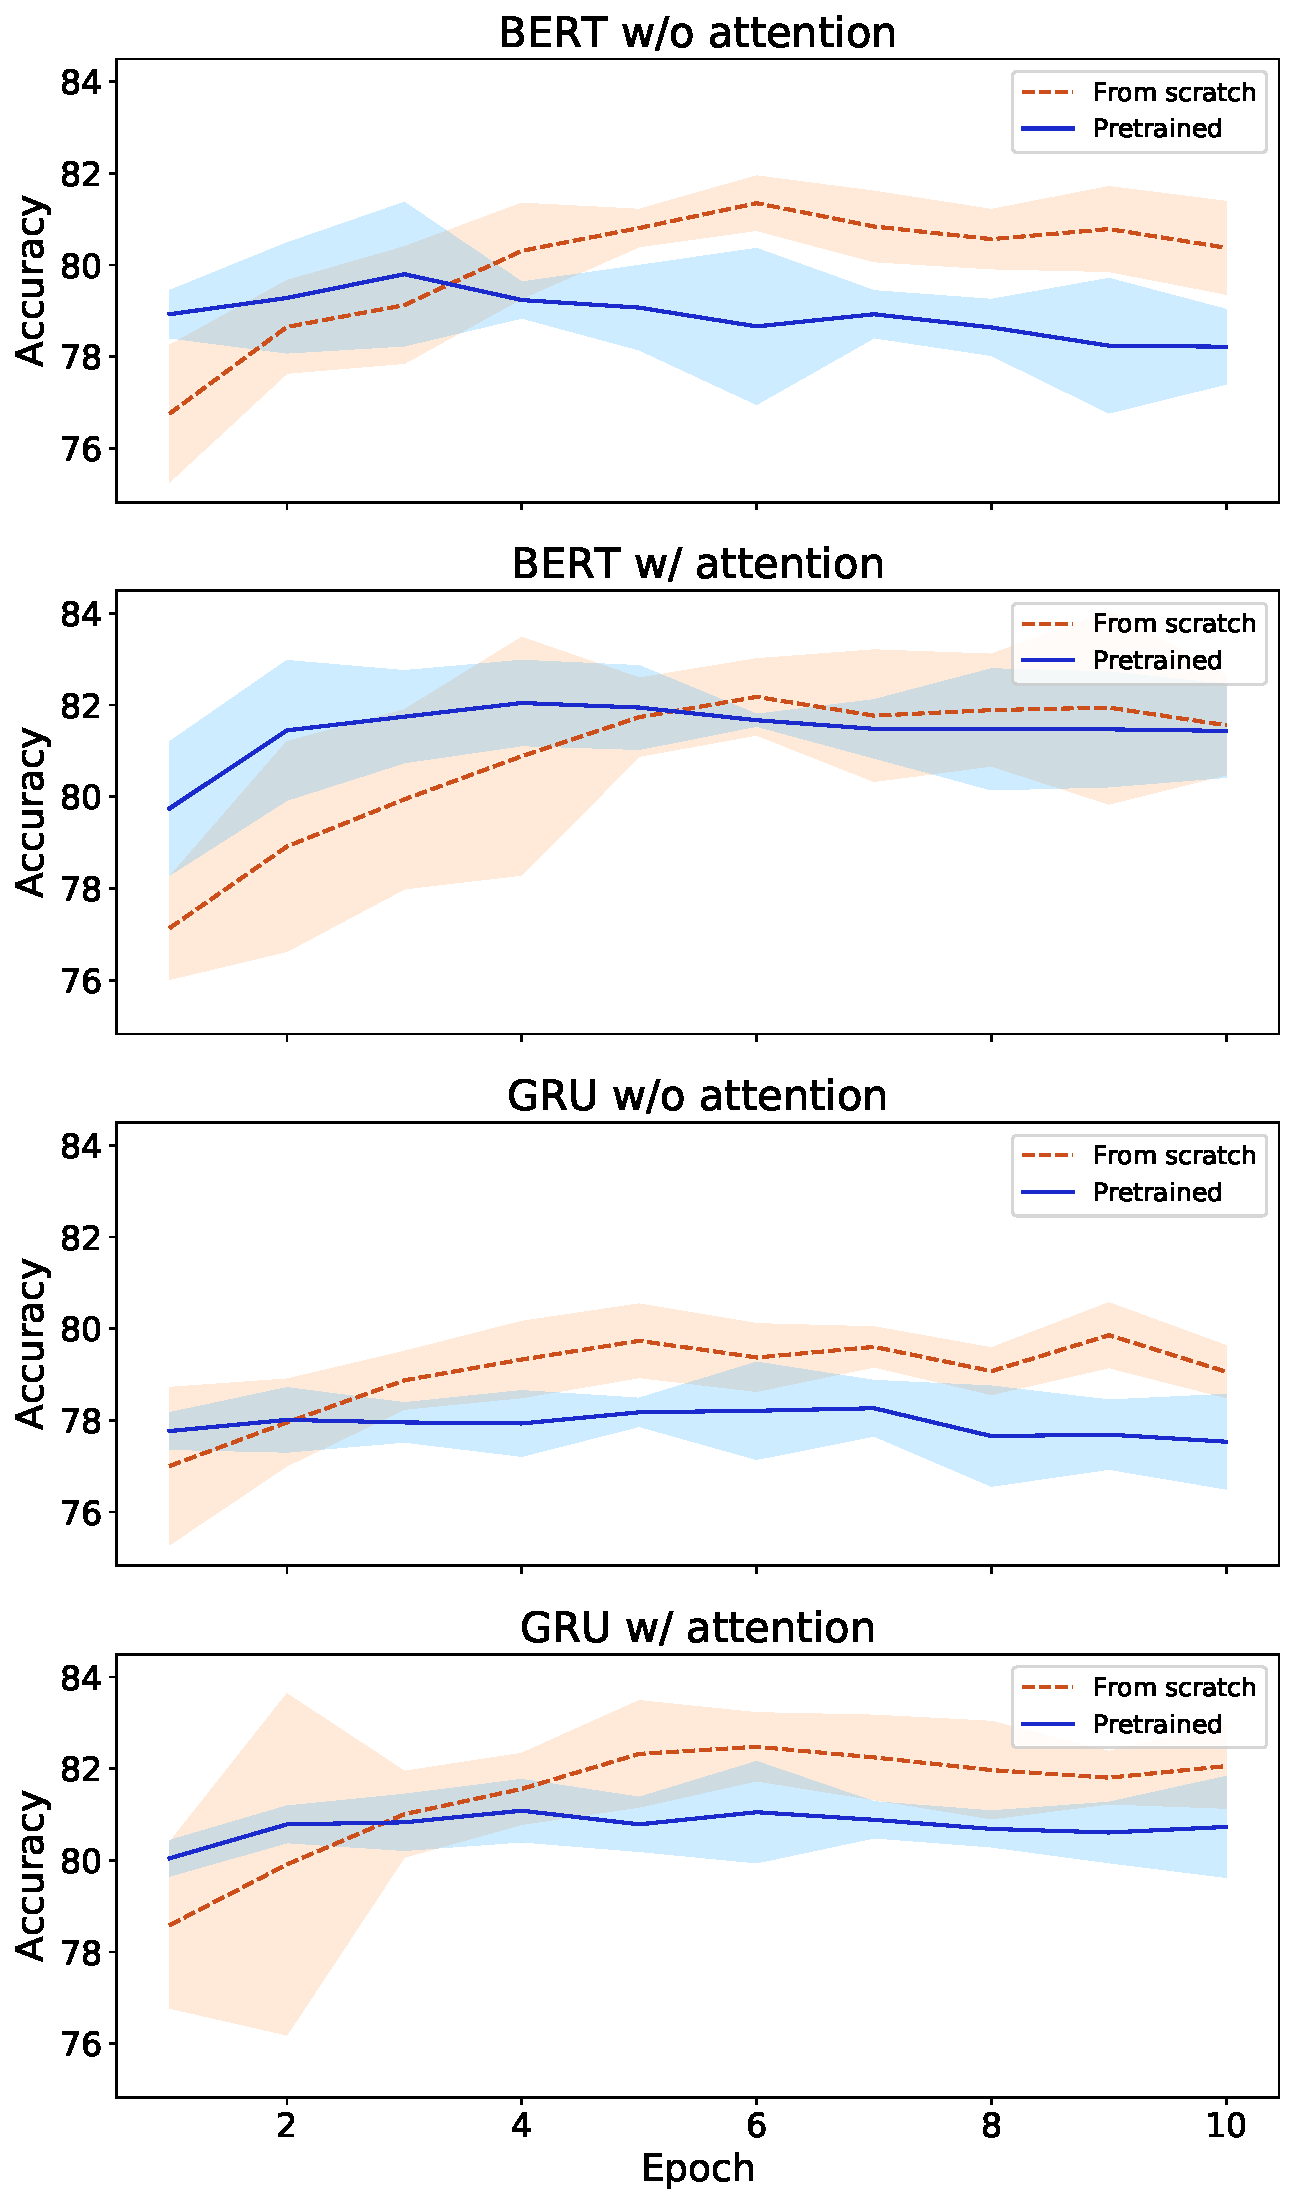
\includegraphics[width=0.8\linewidth]{figures/learning_curves.pdf}
    \caption[Learning curves of transfer learning]{Learning curves of transfer learning. The pre-traning set is synthetic 1.}
    \label{fig:curve}
\end{figure}



\chapter{Discussion}
\section{Improve after deployment}
%[related work]

%An Unsupervised Approach to User Simulation: toward Self-Improving Dialog Systems
%Learning from Dialogue after Deployment - Feed Yourself Chatbot


We propose a framework in this section to discuss the possibility of improving a frame tracking model after its deployment. A deployed dialogue system has the chance of processing through a large number of real dialogues. It would be a huge advantage if we can make use of those data to improve the system. A similar idea is discussed in \cite{hancock2019learning}, where the authors proposed a self-feeding chit-chat dialogue system.
%why? more data, better model
% lifelong learning (Silver et al., 2013) and never-ending (language) learning (Carlson et al., 2010)
In a chit-chat dialogue system, the roles of the user and the system are symmetric. This is not true for a goal-oriented dialogue system, so we adapt their method to fit into our setting.
% (Similar strategy may be used for improving NLU.)

The main idea is to obtain user feedback as frame tracking labels of the corresponding dialogues.
%how to collect user feedback without too much extra effort of a normal user. simple and user-friendly, user experience
There are many ways to achieve this. Here we design a framework that collects active user-feedback while still being user friendly and taking care of user experience.
Due to the time constraint of this project, we don't implement and experiment with this framework.

\subsection{Proposed framework}
%detect low user satisfaction, which means that the system made a mistake in the previous turn
Our system asks for feedback only when the estimated user satisfaction is low, in other words, when it thinks it made a mistake (in the previous turn). Comparing to asking for feedback at every turn, this should reduce the extra effort imposed on a normal user of the system.
% active learning, detect mistake Hashimoto and Sassano (2018)
%ask for correction (in a smart, helpful manner), use the correction from user as feedback labels.
When asking for feedback, the system provides a guess at the same time to be helpful and offer a better user experience. The user feedback is then transformed into training data and labels.

%[example dialogues showing how the system works]

Ideally, in the context of frame tracking, the user feedback would tell us the correct frame reference. This is however infeasible because the concept of frame reference is too complicated to incorporate into a normal dialogue. Instead, correcting or confirming a slot value is more reasonable in terms of the amount of work imposed on the user. So when asking for feedback, the system would pick a slot in the previous turn and ask for correction. This operation is better to be done using natural language rather than an abrupt multiple choice question or a list of options so that the data collection part and the original dialogue are seamlessly combined.

% how to use the feedback: transform user feedback into frame tracking data, and use a multitasking model
This system consists of three tasks. The first one is the frame tracking task.
% satisfaction task
The second one is the satisfaction task, which is used to decide when to ask for feedback. The input of the satisfaction task is the user utterance and the output is a binary class indicating whether the system should ask for feedback or not.
%[write more?]
% feedback task
The last and most important one is the feedback task. The label we have for this task is a slot value in the referred frame, so this is the target we want to predict rather than the frame reference itself as in frame tracking task. However, we still want to make it as similar to frame tracking as possible so that the system can improve on frame tracking when training on feedback data. To account for this, we define the feedback task as follows. The input consists of two parts: the same input as of frame tracking, i.e.\ NLU labels of the current utterance and a list of frames, and the other part is a candidate slot value. The goal of this task is to predict whether the candidate slot value is a correct one, in other words, whether this slot value appears in the referred frame.
% We heavily rely on the assumption that ... slot value <-> frame reference

Inspired by \cite{hancock2019learning}, we propose to combine these three tasks using multitask learning, hoping that training on new feedback data gathered after deployment would improve the performance of frame tracking. Figure \ref{fig:multitask} is an example of a multitask learning model.

%[example of model architecture]
\begin{figure}
    \centering
    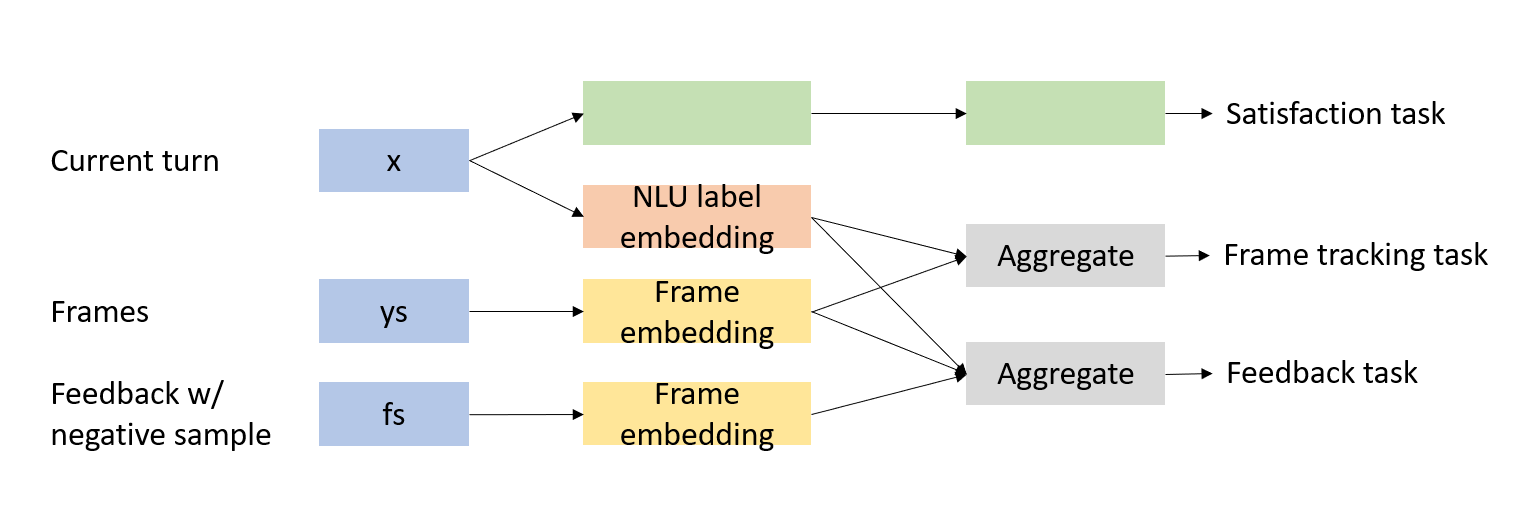
\includegraphics[width=\columnwidth]{figures/multitask2.png}
    \caption[An example of frame tracking after deployment]{Example model for frame tracking after deployment.}
    \label{fig:multitask}
\end{figure}

% the procedure of the pipeline, as a summary
Here we give a procedure of how to create the whole system from scratch.
\begin{enumerate}
    \item Train on Frame tracking task
    \item Collect data for Satisfaction task
    \item Train on Frame tracking + Satisfaction
    \item Deploy and collect data for Feedback task
    \item Train on Frame tracking + Satisfaction + Feedback
    \item Back to step 4.
\end{enumerate}



\chapter{Conclusion}
In this paper, we study how to model memory in a dialogue system using frame tracking. We propose a new model using attention mechanisms to mimic the way humans approach this problem. We evaluate several types of attention mechanisms using the FRAMES dataset. The results give strong evidence of the efficacy of attention, and also show that query-key and scaled query-key are the best mechanisms among the ones we have tried. In addition to the new model, we propose a method to generate synthetic frame tracking data from ordinary dialogues. Experimens show that the training converges faster with model pre-trained on synthetic datasets. As a final touch, we propose a framework for improving a frame tracking model after its deployment.


%----------------------------------------------------------------------------------------
%	THESIS CONTENT - APPENDICES
%----------------------------------------------------------------------------------------

\appendix % Cue to tell LaTeX that the following "chapters" are Appendices

% Include the appendices of the thesis as separate files from the Appendices folder
% Uncomment the lines as you write the Appendices

%\include{Appendices/AppendixA}

%----------------------------------------------------------------------------------------
%	BIBLIOGRAPHY
%----------------------------------------------------------------------------------------

\printbibliography[heading=bibintoc]

%----------------------------------------------------------------------------------------

\end{document}  
